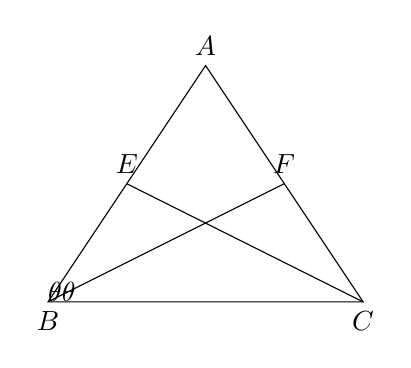
\begin{tikzpicture} 
        \coordinate (A) at (2, 3) {};
        \coordinate (B) at (0, 0) {};
        \coordinate (C) at (4, 0) {};
        \coordinate (E) at (1, 1.5) {};
        \coordinate (F) at (3, 1.5) {};
        \draw (A)node[above]{$A$}--(B)node[below]{$B$}--(C)node[below]{$C$}--cycle;
\draw (B)node[below]{}--(F)node[above]{$F$};
\draw (C)node[below]{}--(E)node[above]{$E$};
\tkzMarkAngle[fill= lightgray,size=0.8cm,%
opacity=.4](C,B,A)
\tkzLabelAngle[pos = 0.6](C,B,A){$\theta$}
\tkzMarkAngle[fill= lightgray,size=0.8cm,%
opacity=.4](A,C,B)
\tkzLabelAngle[pos = 0.6](A,C,B){$\theta$}
\end{tikzpicture}
